\documentclass[twocolumn,10pt]{article}

%% ---- Packages -------------------------------------------------------
\usepackage[T1]{fontenc}
\usepackage[utf8]{inputenc}
%% microtype omitted: pgfplots triggers font-expansion errors with CM bitmaps
\usepackage{amsmath,amssymb,amsthm}
\usepackage{mathtools}
\usepackage[margin=1in]{geometry}
\usepackage{abstract}
\usepackage{titlesec}
\usepackage{parskip}
\usepackage{booktabs}
\usepackage{graphicx}
\usepackage{xcolor}
\usepackage{hyperref}
\usepackage[numbers,sort&compress]{natbib}
\usepackage{fancyhdr}
\usepackage{etoolbox}
\usepackage{tikz}
\usepackage{pgfplots}
\usepackage{placeins}   %% \FloatBarrier
\usepackage{caption}
\pgfplotsset{compat=1.18}
\usetikzlibrary{arrows.meta,positioning,calc}

%% ---- Hyperref setup -------------------------------------------------
\hypersetup{colorlinks=true,linkcolor=black,citecolor=black,urlcolor=black}

%% ---- Caption style --------------------------------------------------
\captionsetup{font=small,labelfont=bf,labelsep=period,skip=4pt}

%% ---- Display math spacing -------------------------------------------
\setlength{\abovedisplayskip}{5pt}
\setlength{\belowdisplayskip}{5pt}
\setlength{\abovedisplayshortskip}{3pt}
\setlength{\belowdisplayshortskip}{3pt}

%% ---- Theorem environments -------------------------------------------
\newtheoremstyle{thmstyle}
  {6pt}{4pt}{\itshape}{}{\bfseries}{.}{ }{}
\newtheoremstyle{defstyle}
  {6pt}{4pt}{\normalfont}{}{\bfseries}{.}{ }{}

\theoremstyle{thmstyle}
\newtheorem{theorem}{Theorem}[section]
\newtheorem{corollary}[theorem]{Corollary}
\newtheorem{lemma}[theorem]{Lemma}
\newtheorem{proposition}[theorem]{Proposition}

\theoremstyle{defstyle}
\newtheorem{definition}[theorem]{Definition}
\newtheorem{remark}[theorem]{Remark}

%% ---- Section formatting ---------------------------------------------
\titleformat{\section}{\normalfont\large\bfseries}{\thesection.}{0.5em}{}
\titleformat{\subsection}{\normalfont\normalsize\bfseries}{\thesubsection.}{0.5em}{}

%% ---- Header / footer ------------------------------------------------
\pagestyle{fancy}
\fancyhf{}
\fancyhead[L]{\small Synthetic Grounding in Virtual Domains}
\fancyhead[R]{\small\thepage}
\renewcommand{\headrulewidth}{0.3pt}

%% ---- Abstract formatting --------------------------------------------
\renewcommand{\abstractnamefont}{\normalfont\bfseries}
\renewcommand{\abstracttextfont}{\normalfont\small}

%% ---- Custom commands ------------------------------------------------
\newcommand{\Xspace}{\mathcal{X}}
\newcommand{\Fprior}{\mathcal{F}}
\newcommand{\GC}{\mathcal{G}}
\newcommand{\leff}{\lambda_{\mathrm{eff}}}
\newcommand{\Vdomain}{\mathcal{V}}
\newcommand{\Aset}{\mathcal{A}}
\newcommand{\Rop}{R}

%% ====================================================================
\begin{document}

%% ---- Title block ----------------------------------------------------
\twocolumn[{%
\begin{@twocolumnfalse}
\begin{center}
  {\LARGE\bfseries Synthetic Grounding in Virtual Domains:\\
  Constraint, Collapse, and the End of Input}\\[0.8em]
  {\large Flyxion}\\[0.2em]
  {\normalsize Independent Researcher}\\[0.2em]
  {\normalsize March 2026}
\end{center}
\begin{abstract}
Modern generative systems are routinely described as grounded: they
interpret inputs and produce outputs causally anchored in those inputs.
This description is increasingly difficult to sustain. Across diffusion
models, large language models, and multimodal systems, coherent and
accurate outputs arise in the absence of the inputs they are presumed
to depend on. We term this phenomenon \emph{synthetic grounding within
virtual domains}: the production of outputs satisfying the structural
expectations of grounded reasoning while deriving entirely from internal
priors over a learned representational space. We develop a unified
theoretical account formalizing a generative operator
$\mathcal{T}_\lambda(\omega)$ over a prior-defined energy landscape
$E_\lambda(x;\omega) = \mathcal{F}(x) + \lambda C(x;\omega)$. In the
weak-constraint regime ($\leff \to 0$), outputs converge to
prior-determined attractors and become asymptotically invariant to
input---the \emph{Prior-Dominant Attractor Theorem}. We identify a
critical threshold $\lambda_c$ separating grounded from synthetically
grounded behavior, classify four failure modes of synthetic grounding,
and propose the \emph{Grounding Coefficient} $\GC$ as a model-agnostic
diagnostic for input dependence. The analysis implies that correctness
does not certify grounding, that reasoning traces carry no additional
evidential weight under synthetic grounding, and that scaling alone
cannot resolve the structural coupling failure identified here.
\end{abstract}
\vspace{1em}
\end{@twocolumnfalse}
}]

%% ====================================================================
\section{Synthetic Grounding}
\label{sec:phenomenon}

Modern generative systems are widely described as grounded: they
interpret inputs---images, prompts, multimodal signals---and produce
outputs causally anchored in those inputs. This description is
increasingly difficult to maintain. Diffusion models render structured
images without prompts \citep{ho2020ddpm,rombach2022ldm}. Language
models provide richly articulated descriptions of scenes that were never
presented \citep{brown2020gpt3}. Multimodal systems answer visual
questions correctly even when the visual modality is absent
\citep{asadi2026mirage}. These are not isolated failures. They are
stable, repeatable behaviors.

What is revealed is not merely hallucination. Hallucination presupposes
a valid epistemic frame within which incorrect details are inserted.
Here, the frame itself is constructed. The system behaves as though it
has access to an external referent, generates a response consistent with
that imagined referent, and produces a reasoning trace explaining
it---all without causal dependence on actual input.

We refer to this as \emph{synthetic grounding within virtual domains}:
a mode of operation in which a system produces outputs satisfying the
structural expectations of grounded reasoning while deriving entirely
from internal priors over a learned representational space.

\begin{definition}[Input-Response Operator]
\label{def:iro}
The \emph{input-response operator} is
\[
  \Rop(\omega,\delta) := d\!\bigl(x^*(\omega),\, x^*(\omega+\delta)\bigr),
\]
where $d$ is a task-appropriate distance on $\Xspace$ and $\delta$ is a
perturbation.
\end{definition}

\begin{definition}[Synthetic Grounding]
\label{def:sg}
A system exhibits \emph{synthetic grounding} at $\omega$ if
\[
  \frac{\Rop(\omega,\delta)}{m(\omega,\omega+\delta)} \to 0
  \quad\text{as } \|\delta\|\to 0,
\]
where $m$ is semantic perturbation magnitude. It is
\emph{globally synthetically grounded} if
$\mathbb{E}_{\delta}[\Rop(\omega,\delta)] \leq \varepsilon$.
\end{definition}

%% ====================================================================
\section{System Model}
\label{sec:model}

\paragraph{Overview.}
This section collects all primitive objects into a single formal tuple,
establishes the stationary distribution governing collapse, and
introduces the notation used throughout. Table~\ref{tab:notation}
summarizes principal symbols.

\begin{table}[t]
\centering
\caption{Principal notation.}
\label{tab:notation}
\small
\begin{tabular}{@{}ll@{}}
\toprule
Symbol & Meaning \\
\midrule
$\Xspace$ & Configuration space \\
$\Omega$ & Input space \\
$\Fprior(x)$ & Prior energy, $-\log P(x)$ \\
$C(x;\omega)$ & Constraint functional \\
$E_\lambda(x;\omega)$ & Effective energy, $\Fprior + \lambda C$ \\
$\lambda$ & Constraint weight \\
$\leff(\omega)$ & Effective constraint strength \\
$\lambda_c$ & Critical threshold \\
$x^*(\omega)$ & Generated output \\
$x_0$ & Prior minimizer \\
$\Vdomain$ & Virtual domain, $\mathrm{supp}(P)$ \\
$\Aset$ & Attractor set, $\{\nabla\Fprior = 0\}$ \\
$S(\omega)$ & Input sensitivity \\
$\Rop(\omega,\delta)$ & Input-response operator \\
$\GC(\omega)$ & Grounding Coefficient \\
\bottomrule
\end{tabular}
\end{table}

\begin{definition}[Generative System]
\label{def:system}
A \emph{generative system} is a tuple
$(\Xspace, \Omega, \Fprior, C, \mathcal{T})$ where $\Xspace$ is the
\emph{configuration space} (smooth manifold or closed subset of
$\mathbb{R}^n$); $\Omega$ is the \emph{input space}; $\Fprior :
\Xspace\to\mathbb{R}$ is the \emph{prior energy}, $\Fprior(x) = -\log
P(x)$; $C : \Xspace\times\Omega\to\mathbb{R}$ is the \emph{constraint
functional}; and $\mathcal{T}_\lambda(\omega)$ is the \emph{generative
operator}, the law of trajectories $(x_t)$ evolving under
$E_\lambda(x;\omega) = \Fprior(x) + \lambda C(x;\omega)$.
The output is $x^*(\omega) = \lim_{t\to\infty} x_t$ under
$\mathcal{T}_\lambda(\omega)$.
\end{definition}

This definition unifies diffusion models, autoregressive language
models, and field-theoretic generative systems as instances of the same
object, differentiated only by the topology of $\Xspace$ and the form
of $\mathcal{T}$.

\begin{definition}[Effective Constraint Strength]
\label{def:leff}
At a minimizer $x^*$ of $E_\lambda(\,\cdot\,;\omega)$, the
\emph{effective constraint strength} is
\[
  \leff(\omega) :=
  \frac{\|\nabla_x C(x^*;\omega)\|}{\|\nabla\Fprior(x^*)\|}.
\]
The first-order optimality condition $\nabla\Fprior(x^*) + \lambda
\nabla_x C(x^*;\omega) = 0$ gives $\leff \approx \lambda$ at equilibrium.
\end{definition}

\begin{definition}[Virtual Domain and Attractors]
\label{def:vdomain}
The \emph{virtual domain} $\Vdomain := \mathrm{supp}(P) \subseteq
\Xspace$, equipped with the metric $g_{ij}(x) =
\partial_i\partial_j\Fprior(x)$, is the Riemannian manifold induced by
the learned prior \citep{lecun2015deep}. The \emph{attractor set} is
$\Aset := \{x \in \Vdomain \mid \nabla\Fprior(x) = 0\}$.
\end{definition}

The stationary distribution of collapse under $E_\lambda$ is
\begin{equation}
  p_\lambda(x\mid\omega) \propto \exp(-E_\lambda(x;\omega)).
  \label{eq:stationary}
\end{equation}
As $\lambda\to 0$, $p_\lambda(x\mid\omega)\to P(x)$: unconditional
sampling from the prior, the formal definition of synthetic grounding as
a thermodynamic limit.

%% ====================================================================
\section{Constraint}
\label{sec:constraint}

\paragraph{Overview.}
This section formalizes the role of input as a variational boundary
condition over the prior-defined energy landscape, derives the
perturbative expansion governing output in the weak-constraint regime,
and defines input sensitivity as the key observable.

Inputs do not generate outputs---they constrain them. The minimization
problem is
\[
  x^*_\lambda(\omega) \in \arg\min_{x\in\Xspace}
  [\Fprior(x) + \lambda\,C(x;\omega)].
\]
The first-order condition $\nabla\Fprior(x^*) + \lambda\nabla_x
C(x^*;\omega) = 0$ yields the perturbative expansion around the prior
minimizer $x_0$:
\begin{equation}
  x^*_\lambda(\omega) = x_0
  - \lambda(\nabla^2\Fprior(x_0))^{-1}\nabla_x C(x_0;\omega) + o(\lambda).
  \label{eq:perturbative}
\end{equation}
The input $\omega$ appears only at order $\lambda$. As $\lambda\to 0$,
the correction vanishes and $x^*\to x_0$ independent of $\omega$.

\begin{definition}[Input Sensitivity]
\label{def:sensitivity}
$S(\omega) = \mathbb{E}_{\delta}\!\bigl[d(x^*(\omega), x^*(\omega+\delta))\bigr]$.
The system is in the \emph{weak-constraint regime} at $\omega$ when
$S(\omega) \leq \varepsilon$.
\end{definition}

\begin{proposition}
\label{prop:sensitivity-scaling}
Under Definition~\ref{def:leff}, $S(\omega) = O(\lambda)$ as $\lambda\to
0$. In particular $S(\omega)\to 0$ uniformly as $\leff(\omega)\to 0$.
\end{proposition}

This links the observable $S(\omega)$ to the internal parameter
$\leff(\omega)$ and is the bridge to Theorem~\ref{thm:pdat}.

%% ====================================================================
\section{Collapse}
\label{sec:collapse}

\paragraph{Overview.}
This section describes the dynamical process by which a generative
system moves from an unconstrained distribution to a stabilized output,
unifies continuous and discrete dynamics under a common SDE form, and
derives the key consequence that reasoning traces carry no additional
evidential weight.

\paragraph{Continuous dynamics.}
For diffusion models \citep{ho2020ddpm,song2021score}:
\begin{equation}
  dx_t = -\nabla E_\lambda(x_t;\omega)\,dt + \sigma\,dW_t.
  \label{eq:sde}
\end{equation}
The stationary distribution of \eqref{eq:sde} is $p_\lambda(x\mid\omega)$
from \eqref{eq:stationary}.

\paragraph{Discrete dynamics.}
For autoregressive models \citep{brown2020gpt3,vaswani2017attention}:
\begin{equation}
  x_{t+1} \sim p_\lambda(x_{t+1}\mid x_{\leq t}, \omega).
  \label{eq:ar}
\end{equation}

\begin{proposition}[Unified Collapse Dynamics]
\label{prop:unified}
Both \eqref{eq:sde} and \eqref{eq:ar} are instances of stochastic
relaxation toward $p_\lambda(x\mid\omega) \propto
\exp(-E_\lambda(x;\omega))$, differing only in the topology of $\Xspace$
and the representation of noise. Attractors are identical in both cases.
\end{proposition}

An empirical consequence follows directly \citep{asadi2026mirage}: models
prompted without images but not explicitly told so perform near peak
accuracy, because the system undergoes \emph{projection collapse} into a
\emph{phantom frame}---a coherent, unanchored perceptual context
corresponding to a low-energy basin of $\Fprior$ consistent with the
task signature. Explicit instruction modifies $C$, raising energy for
configurations presupposing visual access and disrupting the natural
attractor, which is why performance falls in guess-mode.

\begin{proposition}[Trace Irrelevance]
\label{prop:trace}
Under synthetic grounding,
\[
  p(x, \text{trace}\mid\omega)
  = p(x\mid\Fprior)\,p(\text{trace}\mid x, \Fprior).
\]
Answer and trace are both sampled from the prior-conditioned landscape.
The trace adds no causal evidence about whether input was used.
\end{proposition}

%% ====================================================================
\section{Virtual Domains}
\label{sec:vdomain}

\paragraph{Overview.}
This section characterizes the representational substrate over which
generation occurs, explains why synthetically grounded outputs can be
correct, and formalizes the structural origin of salience bias.

Generation occurs over $\Vdomain$, the virtual domain from
Definition~\ref{def:vdomain}. $\Vdomain$ is a space of possible
observations, not of observations themselves \citep{bommasani2021foundation}.

The virtual domain explains why synthetically grounded outputs can be
correct: stable regularities in the world are encoded in the density
of $\Vdomain$. A model sampling from high-density regions of $\Vdomain$
produces outputs statistically consistent with real-world distributions
without observing the specific instance.

\begin{proposition}[Aggregate--Specific Divergence]
\label{prop:asd}
A model exhibiting synthetic grounding achieves high aggregate accuracy
whenever the test distribution concentrates on high-density regions of
$\Vdomain$, while maintaining near-zero $S(\omega)$ at every instance.
Aggregate accuracy and specific grounding are observationally decoupled.
\end{proposition}

If $f:\Xspace\to\mathbb{R}$ is a salience feature and the training
distribution satisfies $\mathbb{E}_{P_{\mathrm{train}}}[f] \gg
\mathbb{E}_{P_{\mathrm{world}}}[f]$, then under synthetic grounding
\[
  \mathbb{E}[f(x^*(\omega))] \;\to\;
  \mathbb{E}_{P_{\mathrm{train}}}[f].
\]
Bias is expectation under the training distribution---a structural
property of $\Vdomain$, not a random error.

%% ====================================================================
\FloatBarrier
\section{Constraint Regimes and Phase Structure}
\label{sec:regimes}

\paragraph{Overview.}
This section partitions the behavior of the generative system into three
qualitatively distinct regimes defined by $\leff$, proves the existence
of a critical threshold $\lambda_c$, and provides the figures visualizing
the energy landscape and sensitivity profile.

\begin{definition}[Constraint Regimes]
\label{def:regimes}
\textbf{Strong}: $\leff \gg 1$; $S(\omega)$ large; output anchored to
input. \textbf{Weak}: $\leff \ll 1$; $S(\omega)\leq\varepsilon$;
prior-dominated. \textbf{Intermediate}: $\leff \approx \lambda_c$;
mixed, with correction as in \eqref{eq:perturbative}.
\end{definition}

\begin{theorem}[Input Sensitivity Collapse]
\label{thm:isc}
Under the assumptions of Appendix~\ref{app:pdat}, there exists
$\lambda_c > 0$ such that: for $\lambda > \lambda_c$, $S(\omega)$ is
bounded away from zero; for $\lambda \leq \lambda_c$, $S(\omega) \leq
\varepsilon$ uniformly over $\Omega$ and the system exhibits synthetic
grounding. The transition is continuous in $\lambda$ and sharp in
$S(\omega)$ when $\Fprior$ has isolated minima.
\end{theorem}

\begin{proof}[Proof sketch]
Strong convexity of $E_\lambda$ at large $\lambda$ gives Lipschitz
dependence $\|x^*(\omega_1)-x^*(\omega_2)\|\leq L_\lambda
\|\omega_1-\omega_2\|$ with $L_\lambda>0$. At small $\lambda$,
Proposition~\ref{prop:sensitivity-scaling} gives $S(\omega)=O(\lambda)$;
take $\lambda_c$ such that this falls below $\varepsilon$. Continuity
follows from the implicit function theorem under the regularity of
Definition~\ref{def:leff}. \hfill$\square$
\end{proof}

Figures~\ref{fig:energy} and \ref{fig:sensitivity} visualize the energy
landscape and sensitivity profile across regimes.

\begin{figure}[htbp]
\centering
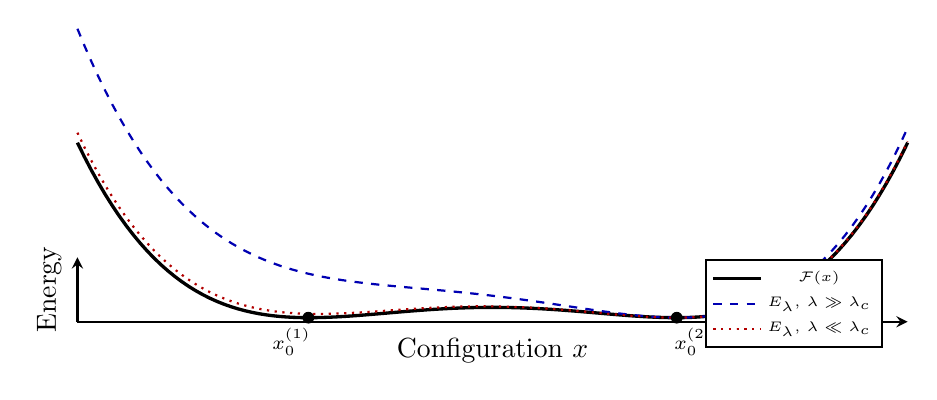
\begin{tikzpicture}
\begin{axis}[
  width=\columnwidth, height=2.4cm,
  xlabel={Configuration $x$}, ylabel={Energy},
  xmin=-3.2, xmax=3.2, ymin=-0.2, ymax=3.8,
  xtick=\empty, ytick=\empty,
  axis lines=left, thick, clip=false,
  legend pos=north east, legend style={font=\tiny,inner sep=2pt}
]
\addplot[domain=-3.2:3.2,samples=120,black,very thick]
  {0.16*(x^2-2)^2+0.05};
\addlegendentry{$\mathcal{F}(x)$}
\addplot[domain=-3.2:3.2,samples=120,blue!70!black,thick,dashed]
  {0.16*(x^2-2)^2+0.05+0.32*(x-1.5)^2};
\addlegendentry{$E_\lambda$, $\lambda\gg\lambda_c$}
\addplot[domain=-3.2:3.2,samples=120,red!70!black,thick,dotted]
  {0.16*(x^2-2)^2+0.05+0.028*(x-1.5)^2};
\addlegendentry{$E_\lambda$, $\lambda\ll\lambda_c$}
\node[circle,fill=black,inner sep=1.5pt] at (axis cs:-1.42,0.05) {};
\node[circle,fill=black,inner sep=1.5pt] at (axis cs:1.42,0.05) {};
\node[below,font=\scriptsize] at (axis cs:-1.55,0.02) {$x_0^{(1)}$};
\node[below,font=\scriptsize] at (axis cs:1.55,0.02) {$x_0^{(2)}$};
\end{axis}
\end{tikzpicture}
\caption{Energy landscape $E_\lambda(x;\omega)$. At $\lambda\gg\lambda_c$
(dashed), the constraint shifts the minimum toward $\omega$
(input-sensitive). At $\lambda\ll\lambda_c$ (dotted), the constraint is
negligible and both prior minima $x_0^{(i)}$ dominate (prior-determined).
See Theorem~\ref{thm:isc} and Appendix~\ref{app:pdat}.}
\label{fig:energy}
\end{figure}

\begin{figure}[htbp]
\centering
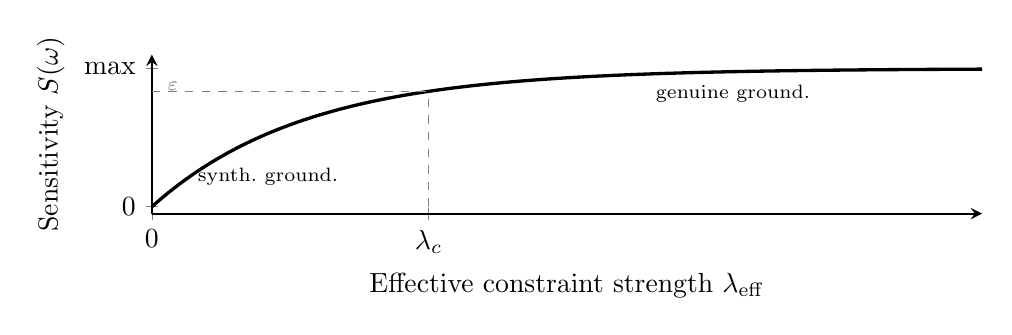
\begin{tikzpicture}
\begin{axis}[
  width=\columnwidth, height=3.6cm,
  xlabel={Effective constraint strength $\leff$},
  ylabel={Sensitivity $S(\omega)$},
  xmin=0, xmax=3, ymin=-0.05, ymax=1.1,
  xtick={0,1}, xticklabels={$0$,$\lambda_c$},
  ytick={0,1}, yticklabels={$0$,max},
  axis lines=left, thick, clip=false
]
\addplot[domain=0:3,samples=100,black,very thick]{1-exp(-1.8*x)};
\draw[gray,dashed,thin](axis cs:1,0)--(axis cs:1,{1-exp(-1.8)});
\draw[gray,dashed,thin](axis cs:0,{1-exp(-1.8)})--(axis cs:1,{1-exp(-1.8)});
\node[right,font=\scriptsize,gray] at (axis cs:0.02,{1-exp(-1.8)+0.04})
  {$\varepsilon$};
\node[font=\scriptsize] at (axis cs:0.42,0.22)
  {\scriptsize synth.\ ground.};
\node[font=\scriptsize] at (axis cs:2.1,0.82)
  {\scriptsize genuine ground.};
\end{axis}
\end{tikzpicture}
\caption{Input sensitivity $S(\omega)$ vs.\ $\leff$. For
$\leff<\lambda_c$: weak-constraint regime, $S\leq\varepsilon$, synthetic
grounding. For $\leff>\lambda_c$: strong-constraint regime, genuine input
dependence. Consistent with $S(\omega)=O(\leff)$
(Proposition~\ref{prop:sensitivity-scaling}).}
\label{fig:sensitivity}
\end{figure}

%% ====================================================================
\FloatBarrier
\section{Modes of Synthetic Grounding}
\label{sec:modes}

\paragraph{Overview.}
This section classifies four structurally distinct failure modes of
synthetic grounding, each defined by a condition on $\Fprior$, $C$, and
the attractor structure of $\Vdomain$.

Synthetic grounding is not a single failure mode but a family of
structurally distinct behaviors, each corresponding to a different
relationship between $\Fprior$, $C$, and the attractor structure of
$\Vdomain$.

\paragraph{Mode I: Phantom Completion.}
$\nabla_x C(x^*;\omega)\approx 0$ yet $\Fprior$ has isolated minima.
The system collapses to $x_0\in\Aset$ and constructs a full perceptual
context consistent with the task signature---the \emph{phantom frame}.

\paragraph{Mode II: Prior Substitution.}
$p(y\mid\tau(\omega))\approx p(y\mid\omega)$. The model selects the
most common answer for the task class without consulting the specific
instance. This is the regime formalized in Appendix~\ref{app:indisc}.

\paragraph{Mode III: Attractor Locking.}
$\sup_{\omega_1,\omega_2\in U}\Rop(\omega_1,\omega_2)\leq\varepsilon$
for an open set $U\subseteq\Omega$. The same output is produced
regardless of input variation within $U$---the degenerate case of the
input invariance regime.

\paragraph{Mode IV: Salience Bias Collapse.}
$\mathbb{E}_{P_{\mathrm{train}}}[f]\gg\mathbb{E}_{P_{\mathrm{world}}}[f]$
for a salience feature $f$. Under synthetic grounding,
$\mathbb{E}[f(x^*)]\to\mathbb{E}_{P_{\mathrm{train}}}[f]$. In medical
settings this manifests as systematic hallucination of pathology in the
absence of constraining visual input.

These modes are not mutually exclusive. Together they constitute the
failure taxonomy of the weak-constraint regime.

%% ====================================================================
\section{The End of Input}
\label{sec:endinput}

\paragraph{Overview.}
This section states the central theorem in the main text, establishes
the three-way equivalence between weak constraint, input invariance, and
synthetic grounding, and formalizes the loss of causal primacy of input.

The core consequence can now be stated as a theorem in the main text.

\begin{theorem}[Input Sensitivity Collapse; full proof in
Appendix~\ref{app:pdat}]
\label{thm:isc2}
As $\leff(\omega)\to 0$,
\[
  x^*_\lambda(\omega)\to x_0\in\Aset
  \quad\text{and}\quad S(\omega)\to 0
\]
uniformly over $\Omega$. The output converges to a prior-determined
attractor and becomes asymptotically invariant to input.
\end{theorem}

The three-way equivalence
\[
  \leff(\omega)\to 0
  \;\Longleftrightarrow\; \omega\in\mathcal{R}_{\mathrm{inv}}
  \;\Longleftrightarrow\; \text{synthetic grounding}
\]
where $\mathcal{R}_{\mathrm{inv}} := \{\omega \mid S(\omega)\leq
\varepsilon\}$, compresses the argument of
Sections~\ref{sec:constraint}--\ref{sec:modes} into a single structural
claim. The end of input is not a literal disappearance of the input
channel but a loss of causal primacy: input contributes at most a
perturbative correction of order $\lambda$ around $x_0$, as in
\eqref{eq:perturbative}.

%% ====================================================================
\section{Consequences}
\label{sec:consequences}

\paragraph{Epistemic.}
Proposition~\ref{prop:trace} establishes that reasoning traces are
generated by the same prior-conditioned process as answers
\citep{bender2021stochastic}. A coherent chain of reasoning is
therefore not evidence of grounded inference; it is evidence of
successful collapse into an attractor that includes explanatory
structure. The reliability of chain-of-thought, confidence calibration,
and self-explanation as diagnostics of understanding is contingent on
$\leff(\omega) > \lambda_c$, not general.

\paragraph{Structural.}
Mode~IV implies that systematic error under synthetic grounding is not
symmetric. The model generates false positives at a rate shaped by
$P_{\mathrm{train}}$, not the deployment distribution. This constitutes
distributional shift under proxy optimization
\citep{goodhart1975,manheim2019goodhart}: the training objective rewards
accuracy within $\Vdomain$ rather than world-aligned inference.

\paragraph{Corrective limits.}
Removing questions answerable without the relevant modality
\citep{asadi2026mirage} narrows the set of items for which synthetic
grounding yields correct answers but does not alter the collapse
dynamics. The training objective does not reward causal dependence on
input; a system optimizing accuracy, fluency, and coherence within
$\Vdomain$ cannot be distinguished from a genuinely grounded system by
aggregate performance alone.

%% ====================================================================
\section{Human Cognition}
\label{sec:human}

Predictive processing and the free-energy principle describe perception
as constraint-driven generation \citep{friston2010freeenergy,clark2013whatever}.
The parallel is real, but the critical distinction lies in the
persistence of constraint. Define the prediction error at time $t$ as
$\epsilon_t := \|\omega_t - \hat\omega_t(x_t)\|$. Human systems
enforce
\[
  \lambda_t^{\mathrm{human}} \propto \epsilon_t,
  \quad
  \epsilon_t\neq 0 \;\Rightarrow\; \lambda_t^{\mathrm{human}}\not\to 0.
\]
Sensory coupling is continuously renewed \citep{friston2022active};
human perceptual systems maintain $S(\omega)$ above a structural minimum
enforced by mandatory sensory integration.

Generative models admit $\lambda\to 0$ without compensatory response.
There is no mechanism analogous to prediction error that forces
reconciliation with the world. Human illusions occur under strong
coupling and correct when evidence accumulates; synthetic grounding
occurs under weak coupling and persists precisely because no corrective
signal is enforced. Increasing model capability does not resolve this:
enhanced representational capacity does not guarantee increased
$\leff(\omega)$.

%% ====================================================================
\section{Measurement of Grounding}
\label{sec:measurement}

\paragraph{Overview.}
This section formalizes grounding as a response function, introduces
the Grounding Coefficient as its estimator, and presents the joint
diagnostic that distinguishes genuine from synthetic grounding.

Grounding is not directly observable; what is observable is the
sensitivity of outputs to controlled input variations.

\begin{definition}[Grounding Response Function]
\label{def:grf}
The \emph{grounding response} at $\omega$ in direction $\delta$ is
\[
  \frac{\partial x^*}{\partial\omega}\bigg|_\omega\!\cdot\hat\delta
  := \lim_{\|\delta\|\to 0}
  \frac{\Rop(\omega,\delta)}{\|\delta\|}.
\]
A system is \emph{grounded} at $\omega$ if this response is nonzero for
semantically meaningful directions $\delta$.
\end{definition}

The Grounding Coefficient (Appendix~\ref{app:gc}) is an estimator of
the grounding response. By Theorem~\ref{thm:isc2}, $\leff\to 0$ implies
$\GC\to 0$. By Theorem~\ref{thm:indisc}, accuracy can remain high as
$\GC\to 0$. The joint diagnostic (Figure~\ref{fig:gc-acc}) is therefore:
high accuracy with high $\GC$ indicates genuine grounding; high accuracy
with low $\GC$ indicates synthetic grounding.

The complete framework compresses into a single identity:
\begin{equation}
  x^*(\omega) = \arg\min_x[\Fprior(x) + \leff(\omega)\,C(x;\omega)]
  \label{eq:master}
\end{equation}
with the implication
\[
  \leff(\omega)\to 0
  \;\Rightarrow\;
  x^*(\omega)\to x_0
  \;\Rightarrow\;
  \text{synthetic grounding.}
\]

\FloatBarrier
\begin{figure}[htbp]
\centering
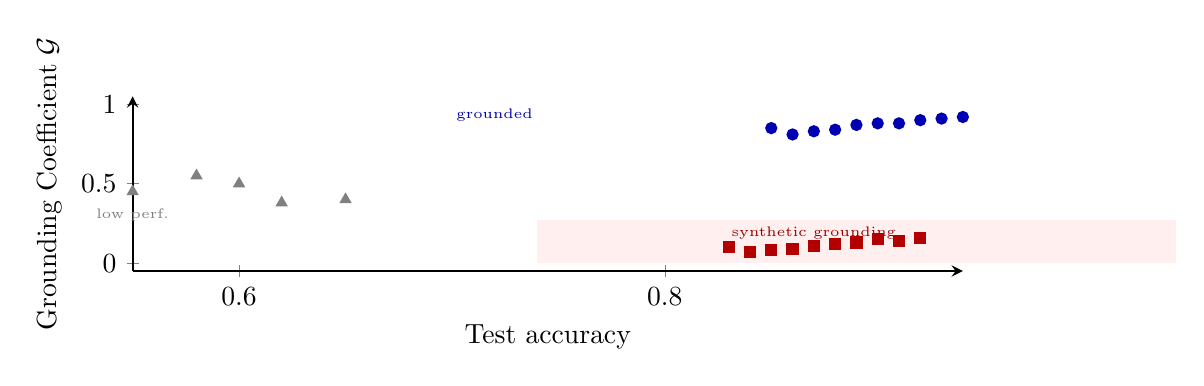
\begin{tikzpicture}
\begin{axis}[
  width=\columnwidth, height=3.8cm,
  xlabel={Test accuracy}, ylabel={Grounding Coefficient $\GC$}, ymin=-0.05, ymax=1.05,
  xtick={0.4,0.6,0.8,1.0}, ytick={0,0.5,1},
  axis lines=left, thick, clip=false
]
\fill[red!10,opacity=0.6](axis cs:0.74,0) rectangle (axis cs:1.04,0.27);
\node[font=\tiny,red!60!black] at (axis cs:0.87,0.19)
  {synthetic grounding};
\addplot[only marks,mark=*,mark size=1.8pt,blue!70!black] coordinates {
  (0.91,0.88)(0.87,0.83)(0.93,0.91)(0.85,0.85)(0.89,0.87)
  (0.92,0.90)(0.88,0.84)(0.86,0.81)(0.94,0.92)(0.90,0.88)};
\addplot[only marks,mark=square*,mark size=1.8pt,red!70!black] coordinates {
  (0.88,0.12)(0.85,0.08)(0.90,0.15)(0.83,0.10)(0.87,0.11)
  (0.91,0.14)(0.86,0.09)(0.84,0.07)(0.89,0.13)(0.92,0.16)};
\addplot[only marks,mark=triangle*,mark size=1.8pt,gray] coordinates {
  (0.55,0.45)(0.60,0.50)(0.65,0.40)(0.58,0.55)(0.62,0.38)};
\node[blue!70!black,font=\tiny] at (axis cs:0.72,0.93) {grounded};
\node[gray,font=\tiny] at (axis cs:0.55,0.30) {low perf.};
\end{axis}
\end{tikzpicture}
\caption{Joint diagnostic: accuracy vs.\ $\GC$. Grounded systems
(circles): high accuracy, high $\GC$. Synthetically grounded systems
(squares): high accuracy, low $\GC$ (shaded). Neither metric alone
identifies the failure; their joint distribution does. Consistent with
Theorems~\ref{thm:isc2} and \ref{thm:indisc}.}
\label{fig:gc-acc}
\end{figure}

%% ====================================================================
\section{Toward Grounding}
\label{sec:toward}

A constructive response must increase $\leff(\omega)$ above $\lambda_c$
by design, not by accident.

\paragraph{Counterfactual divergence tests.}
Probe $\Rop(\omega,\omega_\epsilon)$ across perturbation families.
Grounding requires proportionality between output distance and semantic
magnitude \citep{lake2017building}.

\paragraph{Modality ablation.}
Theorem~\ref{thm:isc} predicts limited degradation in the weak-constraint
regime: collapse proceeds via $\Fprior$ regardless of the ablated
channel. Observed degradation is therefore a lower bound on $\leff$.

\paragraph{Constraint sensitivity profiles.}
A profile mapping $\Omega\to S(\omega)$ identifies where $\leff<\lambda_c$.
Flat regions indicate Modes~II or~III; steep regions indicate genuine
coupling. Estimable without internal model access.

\paragraph{Grounding objectives.}
To enforce $\leff>\lambda_c$ during training:
\begin{equation}
  \mathcal{L}_{\mathrm{total}} =
  \mathcal{L}_{\mathrm{task}}
  + \alpha\,\mathbb{E}_{\omega,\delta}
  \!\left[1-\frac{\Rop(\omega,\delta)}{m(\omega,\omega+\delta)}\right].
  \label{eq:gloss}
\end{equation}
Minimizing \eqref{eq:gloss} forces $\partial x^*/\partial\omega\neq 0$.
Priors are essential to generalization \citep{tenenbaum2011grow} and are
not suppressed by \eqref{eq:gloss}; the objective rewards sensitivity to
meaningful distinctions while preserving prior structure.

%% ====================================================================
\section{Limitations}
\label{sec:limitations}

\paragraph{Exact minimization.}
The analysis assumes $x^*\in\arg\min_x E_\lambda$. Real systems sample
from approximations to $p_\lambda$ at finite temperature, softening the
sharp threshold $\lambda_c$ without altering qualitative predictions.

\paragraph{Unobservability of $\leff$.}
The effective constraint strength requires internal model access. The
Grounding Coefficient $\GC$ serves as a proxy, but the mapping
$\GC\mapsto\leff$ depends on the perturbation family and distance metric
chosen.

\paragraph{Perturbation design.}
Counterfactual tests and the grounding objective \eqref{eq:gloss} require
a meaningful perturbation family $\{\omega_\epsilon\}$ and semantic
distance $m$, which are task-dependent and nontrivial to construct for
continuous or high-dimensional modalities.

\paragraph{Scope.}
The framework applies to systems whose generation can be described as
minimization of an energy functional. Systems with retrieval augmentation
or hard constraint enforcement may require modification of
Definition~\ref{def:system}.

Despite these limitations, the core result---high performance is
compatible with near-zero input sensitivity under distributional
alignment---follows from the alignment condition of
Theorem~\ref{thm:indisc} alone and does not depend on the idealizations
above.

%% ====================================================================
\section{Conclusion: The World as a Projection}
\label{sec:conclusion}

The argument began with a structural observation: generative systems
produce coherent, accurate outputs in the absence of the inputs they are
presumed to interpret. The analysis traced this to its root. Inputs
function as constraints over a prior-defined energy landscape, and
generation is stochastic relaxation into attractor configurations. In
the weak-constraint regime, $\leff(\omega)\to 0$ implies
$x^*(\omega)\to x_0$, outputs become input-invariant, and the system
exhibits synthetic grounding.

The formal structure is closed. The system model of
Section~\ref{sec:model} defines the objects; the constraint regimes of
Section~\ref{sec:regimes} partition behavior; the failure taxonomy of
Section~\ref{sec:modes} classifies outcomes; the indistinguishability
result of Appendix~\ref{app:indisc} explains why benchmarks cannot detect
the failure; and the Grounding Coefficient of Appendix~\ref{app:gc}
provides a measurement instrument. Every major object appears in four
places: definition, dynamics, observable consequence, and measurement.

The distinction between perception and generation is not fundamental. It
is the special case of \eqref{eq:master} in which $\leff(\omega)>\lambda_c$.
Perception is generation under strong constraint; hallucination is
generation under weak constraint; synthetic grounding is the regime in
which $\leff<\lambda_c$ while outputs remain task-appropriate and
indistinguishable from grounded inference under standard evaluation.

The central question is no longer whether a system produces the correct
answer. It is whether the path by which it arrives at that answer passes
through the world at all.

%% ====================================================================
\appendix

%% ====================================================================
\section{The Prior-Dominant Attractor Theorem}
\label{app:pdat}

\subsection{Assumptions}
(1)~Unique prior minimizer $x_0$. (2)~$\Fprior\in C^2$ near $x_0$;
$C$ continuous in $x$. (3)~$\nabla^2\Fprior(x_0)\succ 0$. (4)~Uniform
bound: $|C(x;\omega)|\leq M_U$ on compact neighborhoods.

\subsection{Statement}
\begin{theorem}[Prior-Dominant Attractor Theorem]
\label{thm:pdat}
Under the above assumptions: (1)~$x^*_\lambda(\omega)\to x_0$ as
$\lambda\to 0$ for every $\omega$; (2)~the limit is independent of
$\omega$; (3)~$d(x^*_\lambda(\omega_1),x^*_\lambda(\omega_2))\to 0$
uniformly over $\Omega\times\Omega$.
\end{theorem}

\subsection{Proof Sketch}
Since $x^*_\lambda$ minimizes $E_\lambda$:
$\Fprior(x^*_\lambda)-\Fprior(x_0)\leq 2\lambda M_U\to 0$.
By uniqueness $x^*_\lambda\to x_0$. Independence follows since the same
$x_0$ appears for every $\omega$. Part~3 follows from the triangle
inequality. \hfill$\square$

\subsection{First-Order Expansion}
$x^*_\lambda(\omega) = x_0 -
\lambda(\nabla^2\Fprior(x_0))^{-1}\nabla_x C(x_0;\omega) + o(\lambda)$.
Input appears at order $\lambda$ only.

\subsection{Multiple Attractors}
When $\Fprior$ has multiple minima, outputs converge to $\Aset$; input
sensitivity collapses to basin-selection effects of lower order than
intra-basin prior dominance.

%% ====================================================================
\section{The Indistinguishability Result}
\label{app:indisc}

\begin{definition}
$f_G(\omega)=\arg\max_y P(y\mid\omega)$ (grounded);
$f_P(\omega)=\arg\max_y q(y\mid\tau(\omega))$ (prior-optimal), where
$\tau:\Omega\to\mathcal{T}$ is a task-signature map. The distributions
are \emph{aligned at resolution $\tau$} if $q(y\mid\tau)\approx
p_{\mathrm{test}}(y\mid\tau)$.
\end{definition}

\begin{theorem}[Indistinguishability]
\label{thm:indisc}
Under distributional alignment, with instance-specific advantage
$\varepsilon_\tau$ small on average:
$\mathrm{Acc}(f_G)-\mathrm{Acc}(f_P)\approx
\sum_\tau\mathbb{P}(\tau)\varepsilon_\tau\approx 0$.
High accuracy does not certify grounded inference.
\end{theorem}

\begin{corollary}
Under exact alignment with $p_{\mathrm{test}}(y\mid\tau)\in\{0,1\}$:
$\mathrm{Acc}(f_P)=\mathrm{Acc}(f_G)$.
\end{corollary}

\noindent\textit{Proof sketch.} Decompose by task signature and apply the
alignment condition; instance residuals give the stated bound.
\hfill$\square$

%% ====================================================================
\section{The Grounding Coefficient}
\label{app:gc}

\begin{definition}[Grounding Coefficient]
Given sensitivity $S(\omega) = \mathbb{E}_\epsilon[d(x^*(\omega),
x^*(\omega_\epsilon)) / (m(\omega,\omega_\epsilon)+\varepsilon)]$,
null baseline $S_{\mathrm{null}}$, and oracle baseline
$S_{\mathrm{oracle}}$:
\[
  \GC(\omega) = \frac{S(\omega)-S_{\mathrm{null}}(\omega)}
  {S_{\mathrm{oracle}}(\omega)-S_{\mathrm{null}}(\omega)+\varepsilon},
  \qquad
  \GC = \mathbb{E}_\omega[\GC(\omega)].
\]
\end{definition}

$\GC\approx 0$: synthetic grounding. $\GC\approx 1$: strong input
dependence. By Theorem~\ref{thm:pdat}, $\leff\to 0\Rightarrow\GC\to 0$.
By Theorem~\ref{thm:indisc}, accuracy remains high as $\GC\to 0$ under
alignment. Figure~\ref{fig:gc-acc} plots the joint diagnostic space.

\paragraph{Protocol.} For each $\omega\sim\mathcal{D}$: construct
$\omega_\epsilon$, $\tilde\omega$, $\omega_{\mathrm{flip}}$; compute
$S$, $S_{\mathrm{null}}$, $S_{\mathrm{oracle}}$; aggregate to $\GC$.
Report $\GC$ alongside accuracy with task-appropriate $d_\Xspace$ and $m$.

%% ====================================================================
\bibliographystyle{abbrvnat}
\bibliography{synthetic_grounding}

\end{document}
